\mychapter{8}{Miscellaneous}
\label{chap:misc}
\section{Single-end vs Paired-end \label{sec:SE_vs_PE}}
\begin{wrapfigure}{r}{0.5\textwidth}
  \begin{center}
    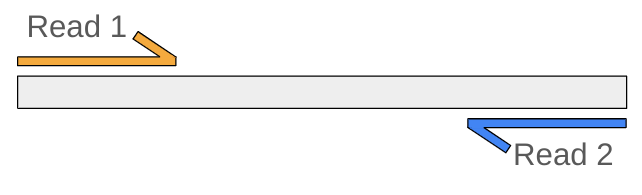
\includegraphics[width=0.5\textwidth]{figures/PE_SE.png}
  \end{center}
  \label{fig:PE_SE}
\end{wrapfigure}
In all pipelines of this toolbox the method of processing of single-end and paired-end sequencing is handle automatically \todo{Are they all adapted?}. However it remains important to understand the difference between these two types of sequencing. The simplest explanation is that single-end (SE) reads/sequences a fragment from a single-end while paired-end (PE) will sequence from both ends. If looking at \autoref{fig:PE_SE} SE would result in only `Read 1' for all fragments while PE would results in both read for each fragment. PE effectively produces twice the amount of reads.\\
The advantage of PE over SE is that PE offers higher quality reads. When sequencing it is expected that the quality of a sequenced read degrades for every base of the fragment (see \autoref{subsec:fastqc_seq_quality}), thus by sequencing from both ends of the fragment we avoid having one end of the fragment being of poor quality. This is particularly useful when we expect fragments to be relatively large, for example in long read RNAseq or in whole genome sequencing. The caveat of PE is that it costs more and requires more computing resources. SE is sufficient for sequencing protocols which generate small fragments such as small RNA-seq as well as sBLISS or Chip-seq.

\section{Glogg \label{sec:glogg}}
Glogg is an application created to browse and search through long or complex files \cite{Glogg}. It was initially designed to look through log files to help programmers find specific locations within a log file, however it can also be used to visualize large genomic files. The search functionality of Glogg is relatively useless for genomic perspectives however visualizing the files allows us to look at it's basic formatting. This is particularly relevant when obtaining Fastq files and checking if it's formatting is compatible with certain tools such as sBLISS \autoref{chap:BLISS_sBLISS}.

\section{Computer terminal \label{sec:terminal}}
The terminal of the computer can be defined in many ways, perhaps the simplest is that the terminal is a direct line of communication from you (the user) to the computer. We consider this a `direct line' as you do not go through a GUI (Graphical User Interface). GUIs are windows which you can scroll, click, and so on. For example, when you want to go to a specific folder and open a file inside it, you will have a window where you can double-click folders and eventually double-click a file to open it. This navigation window is a GUI. That said, the first thing that needs to be known about the terminal is how to navigate through folders.\\
\begin{itemize}
\item Getting a list of files (ls)\\
If you type `ls' in the terminal you will obtain a list of files in your current location.
\begin{lstlisting}
cd seq_toolbox/sbliss/
\end{lstlisting}
\item Changing directories (cd)\\
To change a directory you start by typing `cd' followed by a space and then the name of the directory that you wish to navigate to. The terminal is helpful in the sense that it will assist you with the spelling of your directories/folders. If you hit the `tab' key the terminal will auto-complete as much as possible, if it does not complete the text fully it means that there is more than one possibility. In this case you can hit `tab' twice and it will show you a list of options from the current text. You must then add to the spelling until the remainder of the spelling is unique, at which point you can hit `tab' again and it will autocomplete.\\
The auto-completion when switching looking at folders will only continue to the end of a folder name, the end of a folder/directory is marked by a `/'. At which point you would repeat the previous (type out part of the next folder/file in the sequence and hit `tab').\\
As an example, below I could write out `seq\_' and hit tab, and provided that no other files/folders in my current location start with that name it will complete the entry with `toolbox/', I can then write `sb' and hit `tab' again for it complete the entry with `liss'.\\
Once you have reached your desired location, hit `enter', this will execute the command you have written. In this case your directory will change.
\begin{lstlisting}
cd seq_toolbox/sbliss/
\end{lstlisting}
The above can also be achieved in two separate commands, as seen below.
\begin{lstlisting}
cd seq_toolbox/
cd sbliss/
\end{lstlisting}


\item Navigating backwards or resetting\\
In some instances you may want to go backwards in the directory. One option is to simply write `cd' and hit enter. This will return you to the home directory. An alternative is to write `cd ..' which will go backwards in the directory by one folder. If you were in `A\_projects/seq-toolbox', using `cd ..' will put you in the A\_projects directory.

\item Concatenating files\\
Sometimes a sequencing facility can give fastq files which are separated by lanes. Essentially if the data of one sample is spread on multiple lanes of the sequencer you may obtain as many files as lanes used for that sample. In these instances the files need to be concatenated together. Fortunately there is an easy command to accomplish this, it is appropriately named `cat'. Let's assume we have two files named PFC1\_L3\_1.fq.gz and PFC1\_L3\_2.fq.gz. In this example we know that these two files should be merged together.
\begin{lstlisting}
cd <the directory where the files are located>
cat PFC1_L3_1.fq.gz PFC1_L3_2.fq.gz  > PFC1_L3.fastq.gz
\end{lstlisting}
In the above command we first change the directory to where our files are located. We then call the `cat' command followed by the files we seek to merge, note that this is not limited to two files, one must only ensure that each different file is followed by a space. We then use `>' to indicate the output name, here we will name the product of our merge as `PFC1\_L3.fast.gz'. Upon completion, this new file will be located in the same location as the original files. Note that this does not delete the original files therefore you need to make sure that there is sufficient space/memory on your computer/hard-drive to allow for the creation of this new file.
\end{itemize}

\subsection{Dangers of the terminal}
When using the terminal there are a few things to keep in mind. The most important of which is that a file deleted via the terminal is not recoverable. Files deleted this way are not sent to the trash, they are simply removed. The command to do this is `rm'. For the purpose of this toolbox `rm' will never be required, for this reason I would recommend that those who are unsure of what they are doing DO NOT use the `rm' command. If used incorrectly it is possible to delete key components of a computer's software, thus requiring a full reset of a computer and causing the loss of all data on it.\\
For the curious, if one were to open a terminal, type `rm *' it would delete everything in the current directory. Since the directory in which you open the terminal is the `home' directory, everything save some background folders will be deleted.

\subsection{File permissions}
It is relatively common to encounter errors relating to file permissions, or specifically `permission denied' errors. This translates to a specific file or script not being allowed to read or write in a certain location. This is often due to a file not being considered an `executable', that is a file/process that is supposed to be able to perform an action of some sort, implicitly meaning that it must be able to do changes. To give a file/script the `executable' status we can use a command called chmod which is a shortened version of `change mode'. By using the `+x' parameter we can give a file the `executable' status. Let's say we have a script called `my\_pipeline.sh' which is being denied permission to read/write. We can use the command below to give it the required status/permission. Below we give the +r(read), +w(write) and +x(execute) permissions.
\begin{lstlisting}
cd <the directory where the files are located>
chmod +rwx my_pipeline.sh
\end{lstlisting}
